\thispagestyle{empty} 
\chapter*{\centering Annex 1: Odoo System Overview}
\addcontentsline{toc}{chapter}{Annex 1: Odoo System Overview}
\thispagestyle{empty} 
\textbf{Odoo System Architecture}

Odoo's architecture comprises three main components:

\begin{itemize}
\item \textbf{PostgreSQL Database Server:}
  \begin{itemize}
  \item \textbf{Functionality:} Manages data persistence using an Object Relational Mapping (ORM) layer.
  \item \textbf{Role:} Stores and retrieves structured data necessary for the application's operation.
  \item \textbf{Integration:} Seamlessly integrates with other components to ensure data consistency and reliability.
  \end{itemize}
  
\item \textbf{Application Server:}
  \begin{itemize}
  \item \textbf{Functionality:} Contains business logic, work engine, and output generation.
  \item \textbf{Role:} Executes business processes, calculations, and operations defined by the user and application modules.
  \item \textbf{Scalability:} Scales horizontally to handle increased workload and user interactions.
  \end{itemize}
  
\item \textbf{Presentation Server:}
  \begin{itemize}
  \item \textbf{Functionality:} Allows user access through any web browser (e.g., Chrome, Firefox).
  \item \textbf{Role:} Renders user interfaces, forms, reports, and dashboards based on user interactions and system requests.
  \item \textbf{Customization:} Supports customization of UI through XML-based configurations for views and layouts.
  \end{itemize}
\end{itemize}

\textbf{MVC Architecture Model}

Odoo uses the Model-View-Controller (MVC) design pattern:
   
\begin{figure}[h]
    \centering
    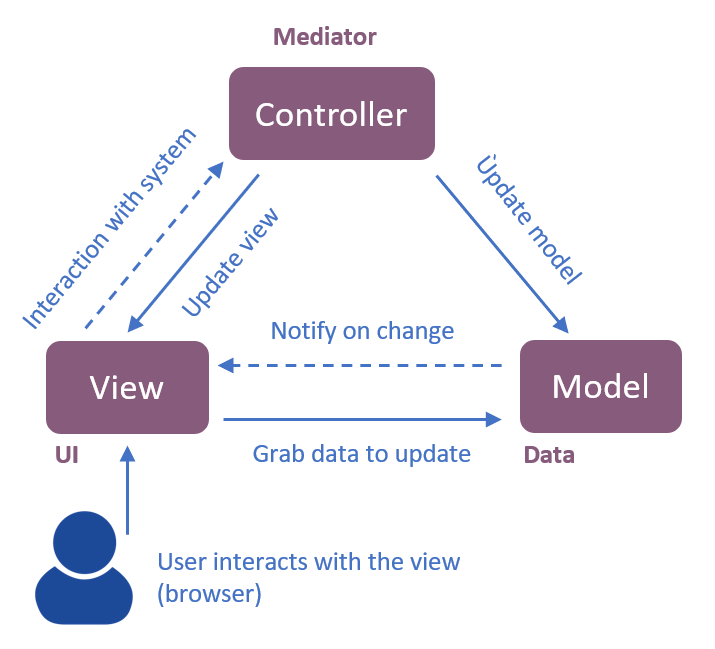
\includegraphics[width=1\textwidth]{media/odoomvc.png}
    \caption{Odoo MVC}
    \label{fig:Odoo MVC}
\end{figure}


\begin{itemize}
\item \textbf{Model:}
  \begin{itemize}
  \item \textbf{Definition:} Defines data structures, entities, and relationships managed by PostgreSQL.
  \item \textbf{Responsibility:} Handles data manipulation, storage, and retrieval operations.
  \item \textbf{Flexibility:} Supports the definition of complex data models tailored to specific business requirements.
  \end{itemize}
  
\item \textbf{View:}
  \begin{itemize}
  \item \textbf{Definition:} Manages user interfaces (UIs), views, and forms presented to end-users.
  \item \textbf{Configuration:} Utilizes XML configurations to define UI components, layouts, and interactive elements.
  \item \textbf{Adaptability:} Enables rapid customization and adaptation of UI elements to meet user preferences and business needs.
  \end{itemize}
  
\item \textbf{Controller:}
  \begin{itemize}
  \item \textbf{Definition:} Controls synchronization, flow, and event management within the application.
  \item \textbf{Execution:} Executes business logic and integrates data processing between models and views.
  \item \textbf{Automation:} Automates workflows and orchestrates complex business processes to enhance operational efficiency.
  \end{itemize}
\end{itemize}

\textbf{Odoo Folder and Module Architecture}

Odoo is modular and flexible, enabling the addition and customization of modules without affecting the entire system:

\begin{itemize}
\item \textbf{Modularity:}
  \begin{itemize}
  \item \textbf{Advantages:} Allows developers to extend functionalities without modifying the core system.
  \item \textbf{Implementation:} Modules are stored in the "addons" directory, ensuring separation from the core application.
  \item \textbf{Flexibility:} Supports the creation of custom modules tailored to specific business needs and requirements.
  \end{itemize}
  
\item \textbf{Customization:}
  \begin{itemize}
  \item \textbf{Flexibility:} Provides the flexibility to add, remove, or update modules independently.
  \item \textbf{Integration:} Ensures seamless integration of third-party modules and custom developments.
  \item \textbf{Deployment:} Facilitates easy deployment of updates and new functionalities without disrupting existing operations.
  \end{itemize}
\end{itemize}
\newpage

% Adding another annex for Scrum methodology
\chapter*{\centering Annex 2: The SCRUM Methodology}
\addcontentsline{toc}{chapter}{Annex 2: The SCRUM Methodology}
\thispagestyle{empty} 
\textbf{Introduction}

\begin{quote}
"Scrum" is a framework for developing complex products. It helps address changing problems while producing high-value products in a productive and creative way. Unlike traditional development methods, Scrum focuses on iterative progress and human resource management.
\end{quote}

\textbf{1. Roles Defined by Scrum:}

\begin{itemize}
\item \textbf{Product Owner:}
  \begin{itemize}
  \item \textbf{Responsibilities:} Defines product requirements and adjusts features during iterations.
  \item \textbf{Role in Development:} Confirms or rejects the partially deliverable version at the end of each sprint.
  \item \textbf{Communication:} Acts as the liaison between stakeholders and the development team.
  \end{itemize}
  
\item \textbf{Scrum Master:}
  \begin{itemize}
  \item \textbf{Responsibilities:} Ensures the correct application of Scrum principles and practices.
  \item \textbf{Conflict Resolution:} Resolves conflicts within the team and facilitates effective communication.
  \item \textbf{Progress Monitoring:} Monitors the team's progress and productivity to optimize workflow.
  \end{itemize}
  
\item \textbf{Development Team:}
  \begin{itemize}
  \item \textbf{Composition:} A multi-skilled, self-organized group of 4 to 6 members.
  \item \textbf{Commitment:} Committed to delivering a potentially shippable product increment at the end of each sprint.
  \item \textbf{Collaboration:} Collaborates closely with the Product Owner to refine requirements and with the Scrum Master to ensure adherence to Scrum practices.
  \end{itemize}
\end{itemize}

\begin{figure}[h]
\centering
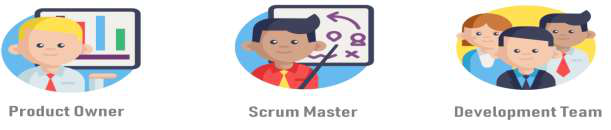
\includegraphics[width=0.7\textwidth]{media/scrum_annex.png}
\caption{Scrum Team Annex}
\label{fig:scrum_team}
\end{figure}

The figure above illustrates the typical structure of a Scrum team, highlighting the roles and interactions among the Product Owner, Scrum Master, and Development Team. Each role contributes to the overall success of the project by leveraging Scrum's iterative approach and collaborative framework.
\thispagestyle{empty} 